%% This is file `elsarticle-template-1-num.tex',
%%
%% Copyright 2009 Elsevier Ltd
%%
%% This file is part of the 'Elsarticle Bundle'.
%% ---------------------------------------------
%%
%% It may be distributed under the conditions of the LaTeX Project Public
%% License, either version 1.2 of this license or (at your option) any
%% later version.  The latest version of this license is in
%%    http://www.latex-project.org/lppl.txt
%% and version 1.2 or later is part of all distributions of LaTeX
%% version 1999/12/01 or later.
%%
%% The list of all files belonging to the 'Elsarticle Bundle' is
%% given in the file `manifest.txt'.
%%
%% Template article for Elsevier's document class `elsarticle'
%% with numbered style bibliographic references
%%
%% $Id: elsarticle-template-1-num.tex 149 2009-10-08 05:01:15Z rishi $
%% $URL: http://lenova.river-valley.com/svn/elsbst/trunk/elsarticle-template-1-num.tex $
%  

%% Use the option review to obtain double line spacing
% \documentclass[preprint,review,12pt,times,authoryear]{elsarticle}
 \documentclass[final,5p,times,twocolumn,authoryear]{elsarticle}

%% Use the options 1p,twocolumn; 3p; 3p,twocolumn; 5p; or 5p,twocolumn
%% for a journal layout:
%% \documentclass[final,1p,times]{elsarticle}
%% \documentclass[final,1p,times,twocolumn]{elsarticle}
%% \documentclass[final,3p,times]{elsarticle}
%% \documentclass[final,3p,times,twocolumn]{elsarticle}
%% \documentclass[final,5p,times]{elsarticle}
%% \documentclass[final,5p,times,twocolumn,authoryear]{elsarticle}

%% if you use PostScript figures in your article
%% use the graphics package for simple commands
%% \usepackage{graphics}
%% or use the graphicx package for more complicated commands
%% \usepackage{graphicx}
%% or use the epsfig package if you prefer to use the old commands
%% \usepackage{epsfig} 

%%------------tables
\usepackage{booktabs} %nice tables i.e. pleasing
\usepackage{rotating}
%\usepackage[nomarkers]{endfloat}
\usepackage{tikz}
%\usetikzlibrary{external}
%\tikzexternalize[prefix=figures/]
\usetikzlibrary{positioning,shapes,arrows,decorations.shapes}
\usepackage{url}
\usepackage{subfigure}

%% The amssymb package provides various useful mathematical symbols
\usepackage{amssymb,amsmath}
%% The amsthm package provides extended theorem environments
%% \usepackage{amsthm}

%% The lineno packages adds line numbers. Start line numbering with
%% \begin{linenumbers}, end it with \end{linenumbers}. Or switch it on
%% for the whole article with \linenumbers after \end{frontmatter}.
\usepackage{lineno}

%% natbib.sty is loaded by default. However, natbib options can be
%% provided with \biboptions{...} command. Following options are
%% valid:

%%   round  -  round parentheses are used (default)
%%   square -  square brackets are used   [option]
%%   curly  -  curly braces are used      {option}
%%   angle  -  angle brackets are used    <option>
%%   semicolon  -  multiple citations separated by semi-colon
%%   colon  - same as semicolon, an earlier confusion
%%   comma  -  separated by comma
%%   numbers-  selects numerical citations
%%   super  -  numerical citations as superscripts
%%   sort   -  sorts multiple citations according to order in ref. list
%%   sort&compress   -  like sort, but also compresses numerical citations
%%   compress - compresses without sorting
%%
%% \biboptions{comma,round}

% \biboptions{}


\journal{Journal of Hydrology}

\begin{document}

\begin{frontmatter}

%% Title, authors and addresses

%% use the tnoteref command within \title for footnotes;
%% use the tnotetext command for the associated footnote;
%% use the fnref command within \author or \address for footnotes;
%% use the fntext command for the associated footnote;
%% use the corref command within \author for corresponding author footnotes;
%% use the cortext command for the associated footnote;
%% use the ead command for the email address,
%% and the form \ead[url] for the home page:
%%
%% \title{Title\tnoteref{label1}}
%% \tnotetext[label1]{}
%% \author{Name\corref{cor1}\fnref{label2}}
%% \ead{email address}
%% \ead[url]{home page}
%% \fntext[label2]{}
%% \cortext[cor1]{}
%% \address{Address\fnref{label3}}
%% \fntext[label3]{}

\title{Input to the Midterm Model}

%% use optional labels to link authors explicitly to addresses:
%% \author[label1,label2]{<author name>}
%% \address[label1]{<address>}
%% \address[label2]{<address>}

\author{Cameron Bracken, Balaji Rajagopalan, Edith Zagona}

\address{}

\begin{abstract}

\end{abstract}

\begin{keyword}
%% keywords here, in the form: keyword \sep keyword

%% MSC codes here, in the form: \MSC code \sep code
%% or \MSC[2008] code \sep code (2000 is the default)

\end{keyword}

\end{frontmatter}


%\linenumbers
%\pagestyle{empty}
%\raggedright


%%%%%%%%%%%%%%%%
%%%%%%%%%%%%%%%%
\section{Introduction}

Every month the United States Bureau of Reclamation (USBR) provides an outlook of reservoir operations in the Upper Colorado River Basin (UCRB) for the following 24 months (\url{http://www.usbr.gov/uc/water/crsp/studies/}).  The outlooks are produced with a RiverWare model known as the 24-Month study (24MS).  The inputs to the 24MS are unregulated reservoir inflows and outflows, starting elevations and storages. The outputs are reservoir storages and elevations for the next 24 months (in some cases the model is run for up to 32 months).  The model takes unregulated flow input since it has very few explicit demands. Unregulated inflow forcasts are generated by the Colorado Basin River Forecast Center (CBRFC). Outflow forecasts are generated colaboratively by reservor operators in both the lower and upper CRB. In early 2010, a model known as the Expanded 24-Month Study (E24MS) as put into use, replacing the original model. This model explicitly represents many demands in the Lower Colorado River Basin (LCRB). Demand inputs are generated by various daily and monthly models run in by the LC region. 

The E24MS like the 24MS before it, can only input a single hydrologic trace (though the inflow is available as an ensemble) and therefore its output is not probablistic. The USBR is able to produce a range of possible outputs by running the model with multiple traces representing the 10th, 50th and 90th percentiles of flow.  This process has been criticized for a number of reasons, one being the considerable effort required to run a single trace, another being that running a 90th percentile trace for example is not a realistic hydologic scenario. 

Also in early 2010, development began on a probabalistic version of the E24MS, know as the Midterm  Operations Model (MOM).  The main feature of this model is built in rules that mimic the operations of each resovoir. This makes it unnecessary to input reservoir outflows.  As a result of the built in operations, an arbitrary number of inflow traces may be run to provide a truely probablisitic look at reservoir conditions over the next 24 months. 

%%%%%%%%%%%%%%%%%%%%%%%%%%%%%%%%%%%%%%%%%%%%%%%%%%%%%%%%%%%%
%%%%%%%%%%%%%%%%%%%%%%%%%%%%%%%%%%%%%%%%%%%%%%%%%%%%%%%%%%%%
\section{Study Area and Data}

\subsection{Study Area}

9 sites in from the UCRB in the MOM. 

\subsection{Constructing a continuous trace}
32 month traces for all for input to the MOM is constructed as a combination of a seasonal forecast model, resampling historical data and a disaggregated hidden Markov (HM) model. A 32 month trace starting on April 1st for a single site is broken down as follows:

\begin{enumerate}
\item {\bf Apr - Jul, Year 1:} From a seasonal forcast model similar to \cite{Bracken:2010cw}.  Output is aggregated to the MOM sites and regression analysis if performed to transform the data from natural to unregualted. In addition Morrow Point and Vallecito need special consideration since they are not present in the natural flow record \cite{Prairie:2005tl}. Morrow Point is constructed as a fraction of Crystal inflow. Vallecito is constructed using regression of Navajo Flow against historical natural flow at Los Pi$\tilde{\mbox{n}}$os.

\item {\bf Aug - Dec, Year 1:} KNN resample \citep{Lall:1995wk} a historical sequence based on the closest the seasonal flow volume. 

\item {\bf Jan - Dec, Year 2:} Using the forecasted seasonal flow volume disaggregate \citep{Nowak:2010ha} from an annual HM model forecast.

\item {\bf Jan - Dec, Year 2:} Same as above but use the second step ahead forecast. 

\item {\bf Jan - Dec, Year 2:} Same as above but use the third step ahead forecast and only include the forst three of 12 months. 
\end{enumerate}

Figure \ref{fig:32} has a schematic of the data inputs

\begin{figure*}
\centering
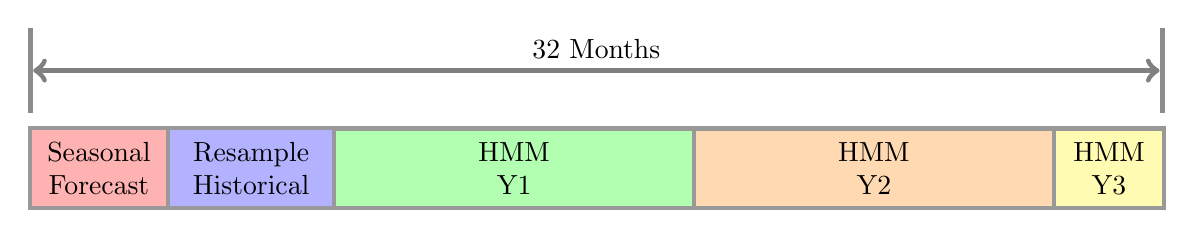
\begin{tikzpicture}[
rec/.style={
    rectangle,
    draw=gray!80,
    align=center,
    anchor=south west,
    inner sep = .5em,
    line width=1.5pt    
    },
line/.style={
    line width=1pt,
    draw=gray!90,
    text width=0pt,
    inner sep=0,
    text height = 3em,
    anchor = south west}
]
\node(seasonal) at (0,0) [rec,text width=4em,fill=red!30] {Seasonal Forecast};
\node(resample) [rec,text width=5em,fill=blue!30] at (5em,0) {Resample Historical};
\node(hmmy1) [rec,text width=12em,fill=green!30] at (11em,0) {HMM\\ Y1};
\node(hmmy2) [rec,text width=12em,fill=orange!30] at (24em,0) {HMM\\ Y2};
\node(hmmy3) [rec,text width=3em,fill=yellow!30] at (37em,0) {HMM\\ Y3};
\node(lleft) at (0,3.5em) [line] {};
\node(lright) [line,anchor=south] at (41em,3.5em) {};
\draw[<->,draw=gray,line width=2pt] (lleft) edge node[above] {32 Months} (lright) ;
\end{tikzpicture}
\caption{Construction of single trace.}\label{fig:32}
\end{figure*}



%%%%%%%%%%%%%%%%%%%%%%%%%%%%%%%%%%%%%%%%%%%%%%%%%%%%%%%%%%%%
%%%%%%%%%%%%%%%%%%%%%%%%%%%%%%%%%%%%%%%%%%%%%%%%%%%%%%%%%%%%
\section{Methodology}

%%%%%%%%%%%%%%%%%%%%%%%%%%%%%%%%%%%%%%%%%%%%%%%%%%%%%%%%%%%%
%%%%%%%%%%%%%%%%%%%%%%%%%%%%%%%%%%%%%%%%%%%%%%%%%%%%%%%%%%%%
\section{Results}

%%%%%%%%%%%%%%%%%%%%%%%%%%%%%%%%%%%%%%%%%%%%%%%%%%%%%%%%%%%%
%%%%%%%%%%%%%%%%%%%%%%%%%%%%%%%%%%%%%%%%%%%%%%%%%%%%%%%%%%%%
\section{Conclusions}


\newpage

\bibliographystyle{elsarticle-num-names}
\bibliography{references}



\end{document}  
